\let\negmedspace\undefined
\let\negthickspace\undefined
\documentclass[journal,12pt,twocolumn]{IEEEtran}
\usepackage{cite}
\usepackage{amsmath,amssymb,amsfonts,amsthm}
\usepackage{algorithmic}
\usepackage{graphicx}
\usepackage{textcomp}
\usepackage{xcolor}
\usepackage{txfonts}
\usepackage{listings}
\usepackage{enumitem}
\usepackage{mathtools}
\usepackage{gensymb}
\usepackage[breaklinks=true]{hyperref}
\usepackage{tkz-euclide} % loads  TikZ and tkz-base
\usepackage{listings}
\usepackage{gvv}
%
%\usepackage{setspace}
%\usepackage{gensymb}
%\doublespacing
%\singlespacing

%\usepackage{graphicx}
%\usepackage{amssymb}
%\usepackage{relsize}
%\usepackage[cmex10]{amsmath}
%\usepackage{amsthm}
%\interdisplaylinepenalty=2500
%\savesymbol{iint}
%\usepackage{txfonts}
%\restoresymbol{TXF}{iint}
%\usepackage{wasysym}
%\usepackage{amsthm}
%\usepackage{iithtlc}
%\usepackage{mathrsfs}
%\usepackage{txfonts}
%\usepackage{stfloats}
%\usepackage{bm}
%\usepackage{cite}
%\usepackage{cases}
%\usepackage{subfig}
%\usepackage{xtab}
%\usepackage{longtable}
%\usepackage{multirow}
%\usepackage{algorithm}
%\usepackage{algpseudocode}
%\usepackage{enumitem}
%\usepackage{mathtools}
%\usepackage{tikz}
%\usepackage{circuitikz}
%\usepackage{verbatim}
%\usepackage{tfrupee}
%\usepackage{stmaryrd}
%\usetkzobj{all}
%    \usepackage{color}                                            %%
%    \usepackage{array}                                            %%
%    \usepackage{longtable}                                        %%
%    \usepackage{calc}                                             %%
%    \usepackage{multirow}                                         %%
%    \usepackage{hhline}                                           %%
%    \usepackage{ifthen}                                           %%
  %optionally (for landscape tables embedded in another document): %%
%    \usepackage{lscape}     
%\usepackage{multicol}
%\usepackage{chngcntr}
%\usepackage{enumerate}

%\usepackage{wasysym}
%\documentclass[conference]{IEEEtran}
%\IEEEoverridecommandlockouts
% The preceding line is only needed to identify funding in the first footnote. If that is unneeded, please comment it out.

\newtheorem{theorem}{Theorem}[section]
\newtheorem{problem}{Problem}
\newtheorem{proposition}{Proposition}[section]
\newtheorem{lemma}{Lemma}[section]
\newtheorem{corollary}[theorem]{Corollary}
\newtheorem{example}{Example}[section]
\newtheorem{definition}[problem]{Definition}
%\newtheorem{thm}{Theorem}[section] 
%\newtheorem{defn}[thm]{Definition}
%\newtheorem{algorithm}{Algorithm}[section]
%\newtheorem{cor}{Corollary}
\newcommand{\BEQA}{\begin{eqnarray}}
\newcommand{\EEQA}{\end{eqnarray}}
\newcommand{\define}{\stackrel{\triangle}{=}}
\theoremstyle{remark}
\newtheorem{rem}{Remark}

%\bibliographystyle{ieeetr}
\begin{document}
%

\bibliographystyle{IEEEtran}


\vspace{3cm}

\title{
%	\logo{
Solution of Q9.3.23
%	}
}
\author{ Anek Anjireddy - EE22BTECH11007
}	
%\title{
%	\logo{Matrix Analysis through Octave}{\begin{center}\includegraphics[scale=.24]{tlc}\end{center}}{}{HAMDSP}
%}


% paper title
% can use linebreaks \\ within to get better formatting as desired
%\title{Matrix Analysis through Octave}
%
%
% author names and IEEE memberships
% note positions of commas and nonbreaking spaces ( ~ ) LaTeX will not break
% a structure at a ~ so this keeps an author's name from being broken across
% two lines.
% use \thanks{} to gain access to the first footnote area
% a separate \thanks must be used for each paragraph as LaTeX2e's \thanks
% was not built to handle multiple paragraphs
%

%\author{<-this % stops a space
%\thanks{}}
%}
% note the % following the last \IEEEmembership and also \thanks - 
% these prevent an unwanted space from occurring between the last author name
% and the end of the author line. i.e., if you had this:
% 
% \author{....lastname \thanks{...} \thanks{...} }
%                     ^------------^------------^----Do not want these spaces!
%
% a space would be appended to the last name and could cause every name on that
% line to be shifted left slightly. This is one of those "LaTeX things". For
% instance, "\textbf{A} \textbf{B}" will typeset as "A B" not "AB". To get
% "AB" then you have to do: "\textbf{A}\textbf{B}"
% \thanks is no different in this regard, so shield the last } of each \thanks
% that ends a line with a % and do not let a space in before the next \thanks.
% Spaces after \IEEEmembership other than the last one are OK (and needed) as
% you are supposed to have spaces between the names. For what it is worth,
% this is a minor point as most people would not even notice if the said evil
% space somehow managed to creep in.



% The paper headers
%\markboth{Journal of \LaTeX\ Class Files,~Vol.~6, No.~1, January~2007}%
%{Shell \MakeLowercase{\textit{et al.}}: Bare Demo of IEEEtran.cls for Journals}
% The only time the second header will appear is for the odd numbered pages
% after the title page when using the twoside option.
% 
% *** Note that you probably will NOT want to include the author's ***
% *** name in the headers of peer review papers.                   ***
% You can use \ifCLASSOPTIONpeerreview for conditional compilation here if
% you desire.




% If you want to put a publisher's ID mark on the page you can do it like
% this:
%\IEEEpubid{0000--0000/00\$00.00~\copyright~2007 IEEE}
% Remember, if you use this you must call \IEEEpubidadjcol in the second
% column for its text to clear the IEEEpubid mark.



% make the title area
\maketitle

\newpage

%\tableofcontents

\bigskip

\renewcommand{\thefigure}{\theenumi}
\renewcommand{\thetable}{\theenumi}

A die is thrown 5 times. Find the probability that an odd number will come up exactly three times.

\solution

\begin{table}[h!]
 \begin{center}
    \begin{tabular}{|l|c|r|}
    \hline
    Parameter & Values & Description\\
    \hline
    $n$ & 5 & Number of throws\\
    \hline
    $k$ & 3 & Number of favourable outcomes\\
    \hline
    $p$ & 0.5 & Probability of getting odd number\\
    \hline
    $X$ & $1\leq X \leq 5$
    & X favourable out of 5 total outcomes\\
    \hline
    $Y$ & $1\leq Y \leq 5$
    & gaussian variable\\
    \hline
    $\mu=np$ & $2.5$ & mean\\
    \hline
    $\sigma=\sqrt{np(1-p)}$ & $1.118$ & standard deviation\\
    \hline
    \end{tabular}
    \end{center}
\end{table}
\begin{enumerate}
   \item{ \em{Binomial Distribution :}}\\The $X$ is the random variable, the pmf of $X$ is given by
    \begin{align}
p_X(k)&=\comb{n}{k}p^k(1-p)^{n-k}
\end{align}    
  We require $\Pr(X = 3)$. Since $n = 5$,
             \begin{align}
                p_X\brak{3} &= 0.3125
             \end{align}
             
             \item{ \em{Gaussian Distribution}}\\
             Let Y be gaussian variable. Using central limit theorem, we can use the gaussian distribution function:
\begin{align}
p_Y\brak{x} &= \frac{1}{\sqrt{2\pi{\sigma}^2}} e^{-\frac{\brak{x-\mu}^2}{2{\sigma}^2}}\\
\end{align}
Using Normal distribution at X=3.
\begin{align}
p_Y\brak{3} &= \frac{1}{\sqrt{2\pi \brak{\frac{5}{4}}}} e^{-\frac{\brak{x-\frac{5}{2}}^2}{2 \brak{\frac{5}{4}}}} \\
&= \frac{1}{\sqrt{2\pi \brak{\frac{5}{4}}}} e^{-\frac{1}{10}}\\
&=0.3228684517
\end{align}
\item {\em{using Q function:}}\\
\begin{align}
	Y \sim \gauss{\mu}{\sigma^2}
\end{align}
The CDF of $Y$:
\begin{align}
F_Y\brak{y} &= 
\begin{cases}
           1-\qfunc{ \frac{y-\mu}{\sigma}}, &  y > \mu \\
           \qfunc{ \frac{\mu-y}{\sigma}} , &  y < \mu
\end{cases} 
\end{align}
But,
\begin{align}
	\frac{Y-\mu}{\sigma} &\sim \gauss{0}{1}\\
	\implies F_Y(y) &= 1 - Q\brak{\frac{y-\mu}{\sigma}}
\end{align}
to include correction of 0.5,
\begin{align}
p_Y\brak{2.5<Y<3.5}&=F_Y(2.5)-F_Y(3.5)\\
&=Q\brak{\frac{2.5-\mu}{\sigma}}-Q\brak{\frac{3.5-\mu}{\sigma}}\\
&=Q\brak{0}-Q\brak{0.8944}\\
&= 0.314446
\end{align}
\end{enumerate}
%Hence we observe that the gaussian and binomial distribution have very less absolute error.
\begin{figure}
\centering
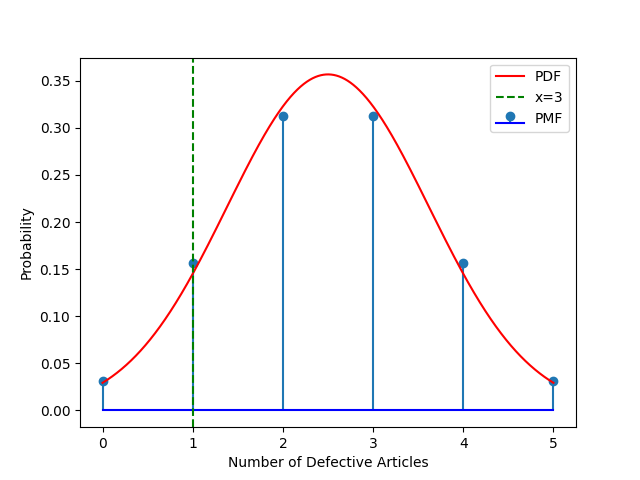
\includegraphics[width=\columnwidth]{./figs/fig1.png}
\caption{ Binomial-PMF and Gaussian-PDFof $X$}
\end{figure}
\end{document}
